\chapter{Architettura}\label{cap:architettura}
Nella specifica del problema (rif. \ref{cap:introduzione}) è stato riportato il funzionamento del sistema da realizzare ei relativi componenti neccessari. Per adempire alle richieste della specifica si è deciso di sviluppare l'applicazione dando priorità ai punti fondamentali, dopodichè sono stati trattati gli aspetti secondari come la taratura dei parametri ei meccanismi di richiesta dei servizi. Nella prossima sezione verrà riportata l'architettura del sistema.
\section{Sistema}
\subsection{Composizione Nodi}
Tutta l'applicazione è stata progettata e sviluppata considerando la presenza di molteplici nodi richiedenti e fornitori, per rendere possibile una simulazione più reale e complessa. Inizialmente sono state prese delle decisioni inerenti la composizione generale di ogni nodo della nostra rete, in particolare si è deciso di supportate nodi di due tipi:
\begin{description}
\item[wired:] nodo fisso collegato tramite cavo;
\item[wireless:] nodo mobile collegato tramite \var{wireless}.
\end{description}
Effettuando tale scelta si sono scatenate un'altra serie di decisioni attinenti l'hardware dei nodi, ovvero l'energia, la memoria ram, il disco e il carico della cpu. Tali componenti sono molto dipendenti dal tipo di collegamento del nodo, in quanto un link di tipo wireless ha bisogno di maggiore calcoli e quindi un utilizzo di energia maggiore.
\begin{figure}[H]
\begin{center}
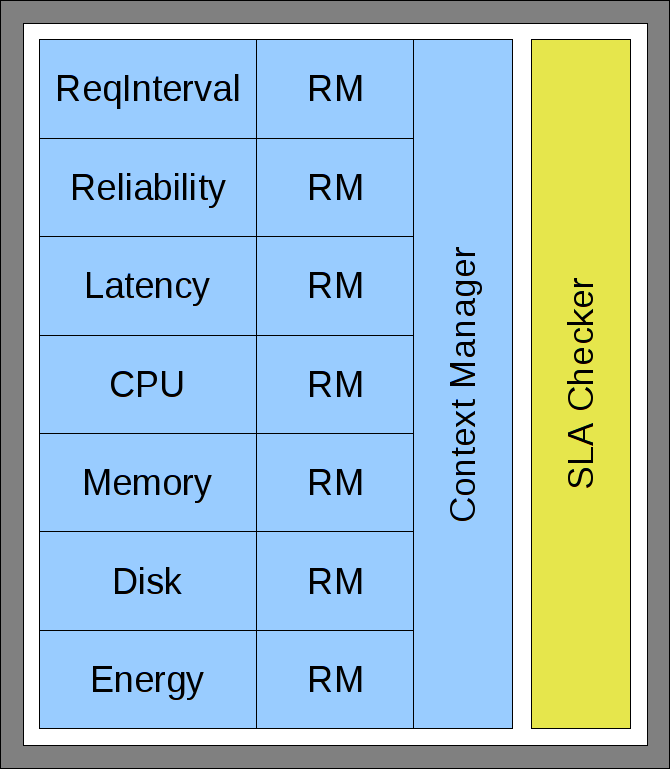
\includegraphics[scale=0.5]{etc/nodo.png}
\caption{Componenti Nodo}
\label{componentinodo}
\end{center}
\end{figure}
Dalla figura \ref{componentinodo} si può notare come è strutturato un singolo nodo, in particolare si può notare come i componenti da monitorare (cpu, memory, disk, energy, latency, reliability, reqInterval) siano in stretto contatto uno a uno con un \var{Resource Monitor}. I \var{Resource Monitor} immettono informazioni dei componenti monitorati sul dsm. Il \var{Context Manager} si occupa di raccogliere tali dati e raggrupparli in un solo oggetto che viene a sua volta immesso sul dsm. Lo \var{SLA Checker} (o \var{SC}), si trova in genere a contatto con il \var{CM} questo perchè raccoglie principalmente le informazioni sul contesto dei vari nodi. Tutte queste parti elencate saranno chiamate d'ora in poi \var{Agenti}, considerando che ci si trova in ambiente di programmazione ad agenti (ovvero \var{Jade}). Gli agenti delle risorse sono stati realizzati per consentire una simulazione più realistica, ovvero ogni agente risorsa non fa altro che generare un valore di utilizzazione basato su vari parametri (ved. cap \ref{cap:modello}).
\subsection{Composizione Rete}
La rete che si è deciso di creare è formata da tanti di questi nodi, sia richiedente che fornitore. Nello specifico ogni nodo fornitore si occupa di fornire un servizio generico, il quale viene registrato nelle pagine gialle del sistema. Ogni richiedente, invece, può richiedere il servizio ad uno qualsiasi dei fornitori disponibili. Questa operazione è stata resa possibile per fare in modo che la simulazione si attenesse ad un tipico caso reale. Per quanto riguarda lo \var{SLA Checker} si è progettato il sistema considerando che tale agente dovesse \var{migrare} da un nodo all'altro in base alle condizioni del contesto. Un esempio della rete in questione con 3 nodi può essere visto in figura \ref{rete}. Si può notare che lo \var{SC} si trova solo su uno dei nodi della rete in quanto deve poter migrare fra di loro.
\begin{figure}[H]
\begin{center}
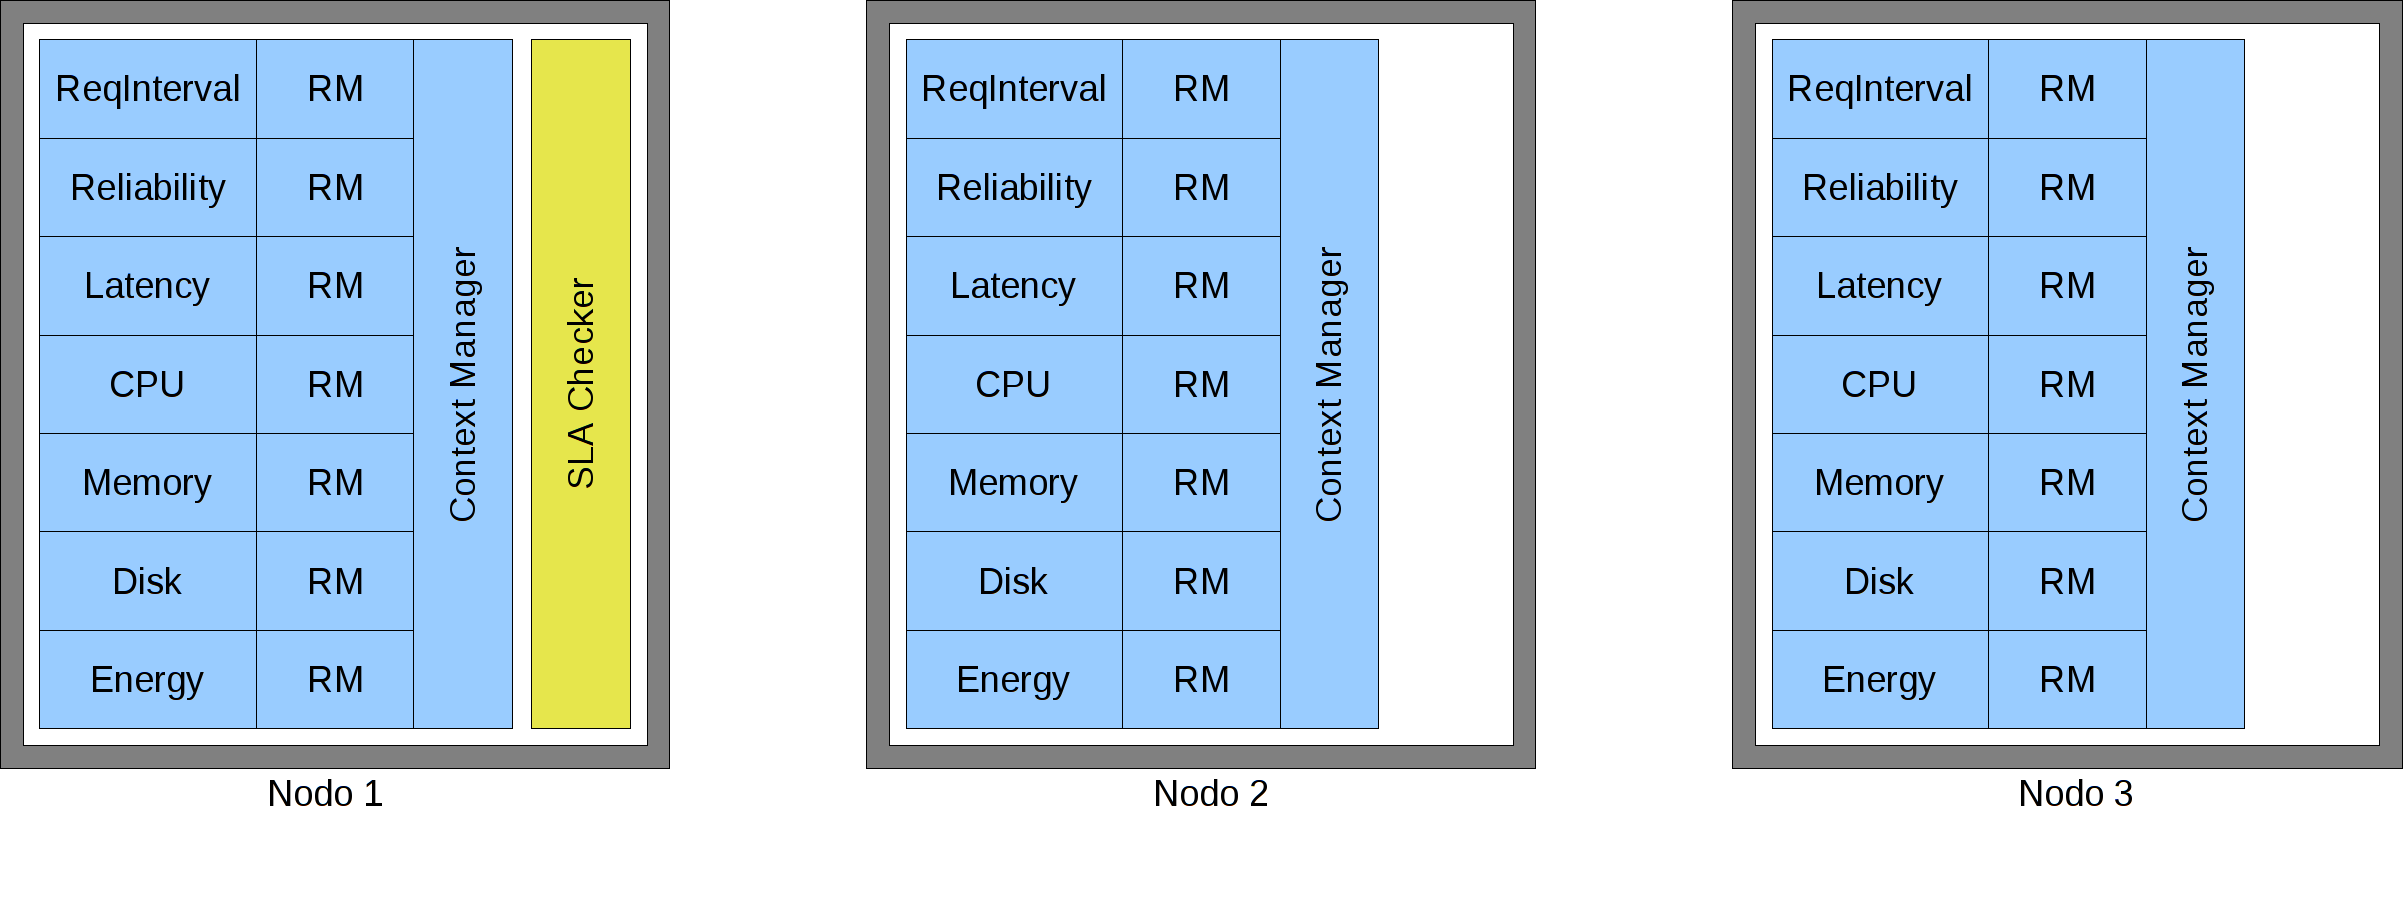
\includegraphics[scale=0.23]{etc/rete.png}
\caption{Esempio di rete con 3 nodi}
\label{rete}
\end{center}
\end{figure}
\section{Funzionamento}
Per spiegare il funzionamento del sistema in questione si è deciso di definire uno scenario d'uso e quindi descrivere il comportamento dei relativi nodi.
\subsection{Scenario d'uso}
Un tipico scenario d'uso potrebbe essere una rete con 3 nodi di cui:
\begin{itemize}
\item 1 nodo fornitore;
\item 2 nodi richiedenti;
\end{itemize}
in particolare ci troviamo in una situazione in cui ognuno dei due nodi richiede un servizio che si attenga al contratto prestabilito con il nodo fornitore. Ogni contratto contiene le seguenti informazioni:
\begin{description}
\item[Publisher:] fornitore del servizio;
\item[Subscriber:] richiedente del servizio;
\item[ReqInterval:] intervallo di tempo tra le richieste del richiedente;
\item[Latency:] tempo impiegato per espletare il servizio;
\item[Reliability:] affidabilità di servizio da parte del fornitore.
\end{description}
Tali informazioni servono per fare in modo che sia il fornitore che il richiedente facciamo il possibile per attenersi ai valori specificati nel contratto.
Su uno dei nodi del sistema è presente lo \var{SLAChecker} che si occupa di controllare la validità di tutti i contratti stipulati; nel caso in cui le condizioni di un contratto vengono violate da uno dei due nodi allora lo \var{SC} informerà immediatamente entrambi i nodi di tale condizione. Tutti i componenti dei nodi sono fortemente dipendenti dalla presenza dello \var{SC}, in quanto comporta un aumento oneroso in termini di calcoli. A causa delle risorse limitate di alcuni nodi (come l'energia) è necessario effettuare un controllo sullo stato attuale dei componenti dei nodi per evitare di sovraccaricarlo, in modo tale che in caso di necessità lo \var{SC} migri su un nodo con condizioni di carico migliori. La selezione del nodo migliore viene fatta utilizzando una specifica politica di selezione (vedi cap. XXX). Un esempio di migrazione può essere visto nelle due figure seguenti, in cui nel primo caso lo SC si trova sul nodo 1, mentre nel secondo caso lo SC è migrato sul nodo 2 a causa di scarsità di risorse sul nodo 1.
\begin{figure}[H]
\begin{center}
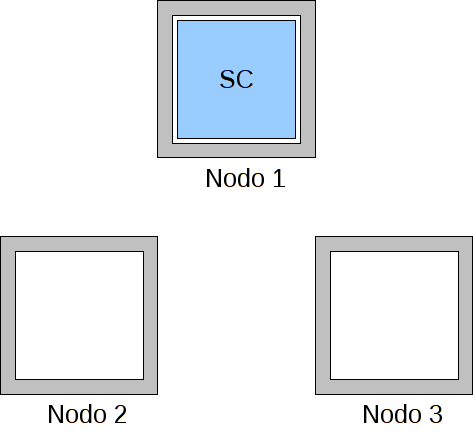
\includegraphics[scale=0.4]{etc/scenario1-1.png}
\caption{Esempio di scenario}
\label{scenario1}
\end{center}
\end{figure}
\begin{figure}[H]
\begin{center}
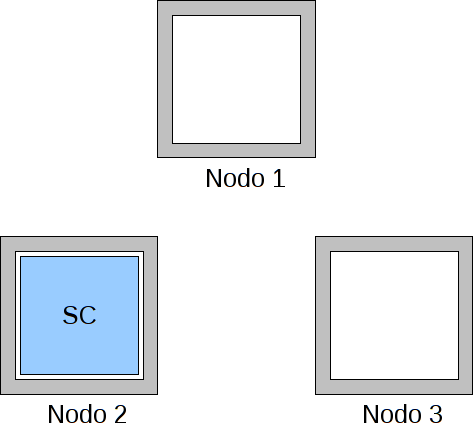
\includegraphics[scale=0.4]{etc/scenario1-2.png}
\caption{Esempio di scenario}
\label{scenario2}
\end{center}
\end{figure}
\subsection{Distribuited Shared Memory}
Per consentire la comunicazione tra i nodi del sistema è stato aggiunto un ulteriore livello nell'architettura in questione, ovvero il \var{dsm}. Tale componente è stato progetto sfruttando i meccanismi di comunicazione di Jade, in particolare lo scambio di messaggi tra server e client dsm avviene tramite messaggi di Jade.
\subsubsection{DsmServer}
E' stato realizzato un agente che si occupa principalmente della ricezione e la computazione delle richieste. Nello specifico quando il server riceve una specifica richiesta effettua la rispettiva operazione sul database dsm.
\subsubsection{DsmData}
Questo componente è necessario per la gestione del dsm e delle tuple, in quanto consente operazioni di \code{IN}, \code{OUT}, \code{UPDATE} e \code{READ}.
\subsubsection{DsmClient}
Quest'ultimo componente è fondamentale per ogni agente che deve inviare o riceve informazioni dal tuple space, infatti consente l'invio delle richieste direttamente all'agente server che provvederà ad esaurirle.
\subsection{Context Manager}
Il Context Manager, come già anticipato, si occupa di raccogliere tutte le informazioni sulle risorse del proprio su un contenitore chiamato \code{Context}, nello specifico il contenuto è il seguente:
\begin{description}
	\item[cpu:] valore del processore;
	\item[ram:] valore della ram presente nel nodo;
	\item[memory:] valore percentuale dell'occupazione di memoria del nodo;
	\item[energy:] valore di energia residua;
	\item[latency:] latenza di trasmissione attuale del nodo publisher;
	\item[reliability:] valore dell'affidabilità del nodo;
	\item[reqInterval:] frequenza di richieste;
	\item[location:] contiene informazioni su cui risiede CM;
	\item[network:] tipo di rete del nodo;
	\item[bandwidth:] banda di rete del nodo.
\end{description}
Per raccogliere tali informazioni il CM effettua delle operazioni di \code{IN} sul dsm ad intervalli predefiniti. Raccolti i dati immette il contesto sul dsm tramite operazioni di \code{OUT}. Il CM si occupa inoltre si richiede ed accettare contratti SLA in base al tipo di nodo in cui si trova, se il nodo è di tipo \var{publisher} accetta contratti invece se è di tipo \var{subscriber} richiede contratti. Una volta accettatto un contratto viene rinviato sul dsm tramite \code{OUT} per essere passato allo SC.
\subsection{SLA Checker}
E' il componente su cui si basa tutto il funzionamento del sistema realizzato, in quanto è l'agente che si occupa di controllare la validità dei contratti e migrare quando necessario. Per effettuare tali operazioni è necessario essere a conoscenza del contesto dei vari nodi e dei contratti SLA stipulati. Lo SC richiede continuamente i contesti dei vari nodi dal dsm, inoltre memorizza tutti i contratti che sono stati stipulati per essere a conoscenza delle relazioni tra i nodi. La conoscenza di tutte le informazioni descritte è necessaria all'algoritmo di \var{checking}, in quanto ha bisogno di tante informazioni per scoprire il miglior nodo su cui migrare (ved. \ref{cap:modello}).